\documentclass[../main.tex]{subfiles}
\graphicspath{{\subfix{../img/}}}

\begin{document}

\section{Materials and Methods} \label{sec:materials_and_methods}

\noindent\textbf{Model.}

Quick intro to Currents

\begin{figure}[H]
    \centering
    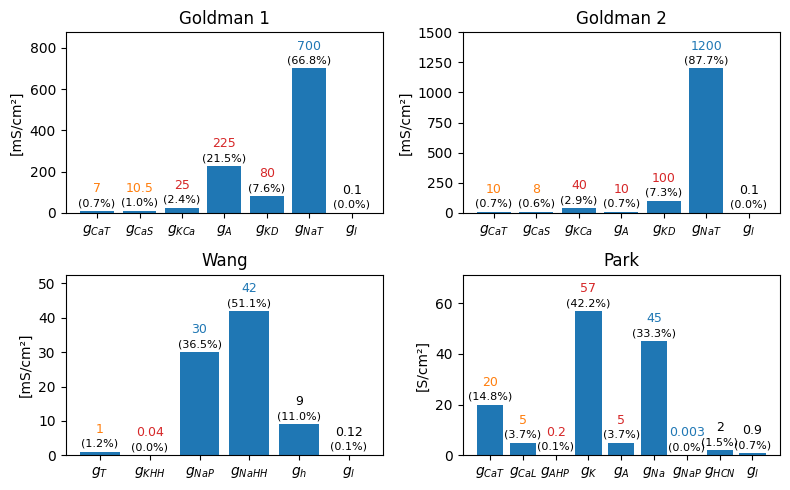
\includegraphics[width=\linewidth]{../img/materials_and_methods/model_conductances.png}
    \caption[Default maximal conductances of the models described]{
        \textbf{Default maximal conductances of the models described.} Labels on the $x$ axis correspond to ion channel names as described in the respective models (see Appendix \ref{appendix:functions_and_parameters} for a detailed description of the models).
        The numbers above each bar indicate the corresponding maximal conductance values, while the percentages below represent their relative value compared to all other channels in the same model.
        Colours indicate the ion permeability of each channel: orange for calcium, red for potassium, blue for sodium, and black for other currents (h-current and leak).
        Among all channels, the \textbf{T-type calcium channels} (labelled as \textbf{CaT} in Goldman and Park models, and \textbf{T} in the Wang model), and \textbf{calcium-activated potassium channel} (labelled as \textbf{KCa} in the Goldman models and \textbf{AHP} in the Park model) are of particular interest in the context of this work. Note that the original Wang model does not include a calcium-activated potassium channel.
    }
    \label{fig:model_conductances}
\end{figure}

\noindent\textbf{Simulations.}

Python and stuff (integration)

Initial conditions - $V=-65$, other variables - steady state.

Simulations were done using python package '\textit{scipy.integrate.solve\_ivp}' with
zero initial conditions. Different integration methods were compared: RK45, BDF, and LSODA.
Each solver is optimized for different problems (stiff, non-stiff, etc.). Simulations
showed, that for some cases (e.g. simulating only t-type channel) it is best to use
RK45. For the simulatins presented in this section, RK45 method was used.

Voltage step protocol: The membrane potential was held at holding potential $-90$ mV,
followed by $150$ms step pulses that varied from $-80$-$40$mV with $10$mV increments
(see e.g. Figure \ref{fig_t_type_ohmic_voltage_traces}, second plot from top). The response
of the neuron to the voltage steps was recorded (see e.g. Figure \ref{fig_t_type_ohmic_voltage_traces}, second figure from top).

\noindent\textbf{Measures.}
Simulated for 40 seconds. First 20 seconds were excluded to allow dynamics to reach stable dynamical regime. Measures were calculated within 20-40 seconds.

Measures: Definition of bursting, bursting period, burst width, interburst interval, intraburst interval, spike width, spiking period

\noindent\textbf{Bifurcation Analysis.}

Auto 07p

Fast-slow decomposition - dynamics of slow subsystem was frozen, fixed points and bifurcations of the rest was computed for each values of the slow variable. Also stability of the fixed points were extracted. Hopf, saddle-node bifurcations and Periodic orbits were obtained.

\noindent\textbf{Fitting Ion Channel Parameters}

As the data from the article is not available online, the values were estimated by taking screenshot, importing the image in Coreldraw and estimating the values using visual inspection and coordinate system of Coreldraw. The fitting was performed using python function \textit{scipy.optimize.curve\_fit}.
The following plots show the estimated activation/inactivation variables, as well as time constants
as a function of test potential $V$, as provided in \parencite{jeongCaa1TFlyTtype2015}:

\begin{note}
    The error due to the subjective visual inspection should not be large. I did not estimated the
    error, but with moving the manually placed dot over the image on the did not have considerable
    effect in the final values (within the moving range where the manually placed dots were not
    obviously not overlapping with the ones from the image).

    The values of the resulted estimates (plotted in the figures above) are provided in
    Section \ref{sec_estimates_of_jeong_2015}.
\end{note}


Parameters for steady-state activation variable were estimated by fitting
$m_{T,\infty}^3(V)$ (see Equation \ref{eq_model_r5_t_type_steady_state_activation}) to the data
from electrophysiological recordings presented in \parencite{jeongCaa1TFlyTtype2015} (similar to
the procedure described in \parencite{coulterCalciumCurrentsRat1989}). The steady-state inactivation
was estimated by fitting Equation \ref{eq_model_r5_t_type_steady_state_inactivation} to the
data from the same paper.

I-V relationship

\end{document}